\documentclass[../../main.tex]{subfiles}
 
\begin{document}

\begin{table}
\small
\centering
\begin{tabular}{| c | c | c | c | c | c | c |}
\hline \hline
Question & 135A $N$ & 135A Mean & 135A Std. dev. & 135B $N$ & 135B Mean & 135B Std. dev. \\ \hline
10 & 21 & 3.76 & 1.04 & 18 & 3.72 & 0.96 \\ \hline
11 & 21 & 4.57 & 0.75 & 18 & 4.78 & 0.43 \\ \hline
12 & 21 & 4.29 & 1.01 & 18 & 3.78 & 1.00 \\ \hline
13 & 21 & 3.52 & 1.33 & 18 & 3.33 & 1.53 \\ \hline
14 & 21 & 3.48 & 1.36 & 18 & 2.72 & 1.32 \\ \hline
15 & 21 & 3.29 & 1.68 & 18 & 2.28 & 1.53 \\ \hline
16 & 21 & 3.19 & 1.57 & 18 & 2.94 & 1.30 \\ \hline
\hline
\end{tabular}
\caption{\label{tab:courses:intro_eval_1} Summary of questions 10-16 on the student evaluation form, for PHYS135A/B taught in Fall 2017 and Spring 2018.  These questions pertain to the \textit{course}.}
\end{table}

\begin{table}
\centering
\begin{tabular}{| c | c | c | c | c | c | c |}
\hline \hline
Question & 135A $N$ & 135A Mean & 135A Std. dev. & 135B $N$ & 135B Mean & 135B Std. dev. \\ \hline
17 & 21 & 4.24 & 1.04 & 18 & 3.67 & 1.03 \\ \hline
18 & 21 & 3.52 & 1.33 & 18 & 3.11 & 1.57 \\ \hline
19 & 21 & 3.48 & 1.40 & 18 & 2.89 & 1.29 \\ \hline
20 & 21 & 4.24 & 1.09 & 18 & 4.06 & 1.25 \\ \hline
21 & 21 & 4.48 & 1.03 & 18 & 3.78 & 1.17 \\ \hline
22 & 21 & 4.10 & 0.89 & 18 & 3.88 & 1.02 \\ \hline
23 & 21 & 3.95 & 1.20 & 18 & 3.53 & 1.33 \\ \hline
24 & 21 & 4.67 & 0.58 & 18 & 4.24 & 0.97 \\ \hline
25 & 21 & 3.24 & 1.55 & 18 & 3.12 & 1.36 \\ \hline
\hline
\end{tabular}
\caption{\label{tab:courses:intro_eval_2} Summary of questions 17-25 on the student evaluation form, for PHYS135A/B taught in Fall 2017 and Spring 2018.  These questions pertain to the \textit{professor}.}
\end{table}

Tables \ref{tab:courses:intro_eval_1} and \ref{tab:courses:intro_eval_2} show the results of the \textit{algebra-based} introductory physics courses taught in the 2017-2018 academic year.  Tables \ref{tab:courses:intro_eval_3} and \ref{tab:courses:intro_eval_4} show the results of the \textit{calculus-based} introductory physics courses taught in the 2017-2018 academic year.  The results show an interesting correlation that reveals a potential strategy for continual improvement of my teaching in these courses. \\ \hspace{0.1cm}

First, there are areas that need improvement.  Questions 14-16 and 19 read as follows: ``This course improved my understanding of the material,'' ``This course increased my interest in the subject matter,'' ``Overall, I would recommend this course to others,'' and ``The professor was able to explain complicated ideas,'' respectively.  For \textit{algebra-based physics}, there are no pre-requisite courses, but students are required to solve problems involving algebraic equations, graphical analysis, and concepts like vectors and vector fields.  It is not surprising that students struggle if they're encountering these concepts for the first time.  I have been trained to teach much faster than the students who disapproved expected.  \\ \hspace{0.1cm}

In the students' written responses, the most common remark was that the pace of the course was too fast, and that they desired more traditional lecture time with explicit examples given.  Some students remarked that the portions of the lecture on the projector (e.g. PI-modules, JITT-modules) were not as helpful as the traditional style with examples.  In Fall 2017, Professor Serkan Zorba and I both taught PHYS135A, and in Spring 2018 we both taught PHYS135B, meaning that some students had to switch professors.  Students who switched were newly stressed by the increased pace, in addition to the students I had from the Fall.  Some students even met with me in office hourse to brainstorm ways in which we could move more slowly, but still cover the necessary book chapters. \\ \hspace{0.1cm}

PHYS135B introduces the concept of vector \textit{fields}, necessary for understanding electromagnetic fields.  This new concept further added difficulty for students encountering vectors for the first time\footnote{A single vector describes, for example, the velocity of a single leaf blown in a direction by the wind.  A vector field, on the other hand, describes the wind velocity at all points in space.}.  The research-based methods such as PI-modules rely on groups of students teaching each other.  If a whole group is struggling, they don't gain the benefit of the one student who understands the problem to show them how to solve it.  Thus, the average scores on questions 14, 16 and 19 showed slight decreases (less than one standard deviation).  I assess this further below in the discussion of Fig. \ref{fig:ag_data}.  Responses to Question 11, ``This course was academically challenging'' showed a slight increase, which is evidence that the students found the second semester more difficult than the first.  \\ \hspace{0.1cm}

I did not encounter many written responses in which students expressed strong feelings about question 15, ``This course increased my interest in the subject matter.''  Most students taking PHYS135A/B are fulfilling a requirement for their major (a two-thirds majority are KNS majors), and typically do not express a strong desire to take the course\footnote{Question 9: ``I had a strong desire to take this course.'' PHYS135A/B students reported $3.24\pm 1.64$ and $3.00\pm 1.71$, respectively.}.  Nevertheless, I have attempted to add content that appeals to KNS majors.  For example, when we reach concepts in PHYS135A pertaining to biomechanics, such as torque, I give specific example problems and final project assignments that relate in some way to torque in the human body.  Another example pertains to PHYS135B, which addresses electric current.  When we reach the topic of current, the class solves problems specific to the electrical currents in the human nervous system\footnote{In the supplemental materials I include a student's final presentation on the electrical nerve activity of a bicep under torque.}.  For more information on KNS-relevant material in PHYS135A/B, see Sec. \ref{sec:future}. \\ \hspace{0.1cm}

In \textit{calculus-based physics}, the story was different.  There are many areas in which the courses and my teaching scored well.  \textbf{I am especially proud of the fact that Q25 (``Overall, I would recommend this professor to others'') jumped in 2018 relative to 2017 for the calculus-based courses.  In fact, my teaching scores improved in every single category in calculus-based physics in going from Fall 2017 to Spring 2018.}  Further, students in both sections believed that the courses were rigorous and challenging, while still giving me increasing marks in all categories.  Some students appreciated the PI modules, PhET simulations, and JITT exercises.  This is reflected in responses to question 12 on the standard evaluation (``This course offered useful learning tools''), which is a key data point.  I focus on this data point because I am being asked by my department to teach in an activities based style with modules like PI-modules, different from the traditional lecture.  The purpose of the activities and group exercises is to satisfy the focus on \textbf{improvement of analysis skill}.  The PI, JITT, and PhET modules are constructed to improve analysis skill through conceptual understanding.  However, upon reflecting on the students' constructive comments, it seems that these modules benefit some students but not all. \\ \hspace{0.1cm}

A vital teaching method emerged in PHYS180, which the students call ``board problems'' in their written responses to evaluations.  It started with an interesting compromise between my desire to move forward in the book faster, and the students' desire to go slowly and have me do examples.  Notice that in the PHYS180 written responses, the students still express quite often a desire for worked examples in class.  In light of all the research-based teaching methods that encourage students to learn through interactions with each other, I decided to have them \textit{work example problems for each other}.  I began by giving an example problem to the class.  The problem would be difficult, and I would either design it myself, or draw it from the current chapter.  Students would then work the problem in groups of 3-4 on the whiteboards, next to other groups.  The class responded positively to this method, and it is reflected in their written responses.  Some even state explicitly that my teaching improved!  The board-problem method works for two reasons: it allows struggling students to see how harder problems are approached by peers, and struggling groups see other groups' strategies and therefore learn from the whole class.  \\ \hspace{0.1cm}

In addition to the inclusion of board-problems, I have reflected on my student evaluations and have decided on \textbf{three concrete improvements} to my introductory courses.  In consultation with my department chair, and in studying past PEGP documents in my department, the first improvement will be an increase in traditional lecture content.  The reason is that if every single concept and number in physics is confusing to a first-time student, then merely updating the teaching style with researched-based modules will not help that student.  The traditional lecture style offers the benefit that students see many example problems done in explicit detail, such that they can copy and repeat the technique.  I was taught to never expect this as an undergraduate student.  My colleagues in my department have reassured me that it is necessary to give inexperienced students an explicit starting point.  Thus, going forward in my introductory courses, \textit{a significant fraction of class-time will be spent on concrete examples in the traditional style.} \\ \hspace{0.1cm}

The second major change I will be making to my introductory course teaching style is to slow the pace.  In reading students' remarks, this is the second most common desire on their part.  I was taught at the undergraduate and graduate levels at high speed, with intense focus on both content and mathematical detail.  Of course I must make adjustments for the environment at Whittier College, and not merely teach to myself.  I must \textit{teach to the middle}, as one of my colleagues recommended.  The students felt relief when I began assigning them board-problems, precisely because it allowed them to slow down, and check their work with each other and other groups.  Thus, the addition of board-problems solved both the problem of pace and example problems at once.  The students got a chance to lecture to each other momentarily.  In the upcoming semester, \textit{I will include the group-board technique in the normal course plan}. One minor adjustment to this technique is that the courses are getting larger enrollments, and we may run out of whiteboard space.  My planned response to this is to sketch the problem myself, and then allow student groups to design specific examples meant to be exchanged among the groups.  So far this has worked in my Fall 2018 PHYS135A sections when it's not feasible to do board-problems.  \\ \hspace{0.1cm}

The third change I'd like to make is to include more applications of calculus in the \textit{calculus-based} introductory sequences.  In my view, more applications of calculus should be included in PHYS150/PHYS180.  From the feedback from my department, I need to include more laboratory activities in PHYS180.  Thus, I propose solving both problems simultaneously.  When I teach \textit{calculus-based} introductory courses in the future, I will use the laboratory activities as a venue for demonstrating the difference between results obtained from calculus (derivatives and integrals) and the average results one obtains without calculus. It is my hope that the students will learn to use some calculus tools, even if the majority cannot deploy calculus in some challenging homework problems.  The assumption that a majority of students concurrently taking calculus would recognize the same concepts in physics was likely part of the discussion about the pace of the courses.  Howerver, the inclusion of more lab activities is mandatory (and now possible because I'm fully trained on all the equipment). Thus including calculus concepts in the labs will require little extra effort. \\ \hspace{0.1cm}

\begin{table}
\small
\centering
\begin{tabular}{| c | c | c | c | c | c | c |}
\hline \hline
Question & 150 $N$ & 150 Mean & 150 Std. dev. & 180 $N$ & 180 Mean & 180 Std. dev. \\ \hline
10 & 16 & 4.19 & 0.83 & 18 & 4.00 & 0.91 \\ \hline
11 & 16 & 4.19 & 1.38 & 18 & 4.67 & 0.49 \\ \hline
12 & 16 & 3.63 & 1.31 & 18 & 4.06 & 0.94 \\ \hline
13 & 16 & 4.00 & 1.10 & 18 & 4.00 & 0.97 \\ \hline
14 & 16 & 3.93 & 1.33 & 18 & 3.89 & 0.90 \\ \hline
15 & 16 & 3.56 & 1.26 & 18 & 3.67 & 1.03 \\ \hline
16 & 16 & 3.56 & 1.26 & 18 & 3.83 & 0.86 \\ \hline
\hline
\end{tabular}
\caption{\label{tab:courses:intro_eval_3} Summary of questions 10-16 on the student evaluation form, for PHYS150 taught in Fall 2017, and PHYS1809 taught in Spring 2018.  These questions pertain to the \textit{course}.}
\end{table}

\begin{table}
\centering
\begin{tabular}{| c | c | c | c | c | c | c |}
\hline \hline
Question & 150 $N$ & 150 Mean & 150 Std. dev. & 180 $N$ & 180 Mean & 180 Std. dev. \\ \hline
17 & 16 & 3.31 & 1.14 & 18 & 3.44 & 1.15 \\ \hline
18 & 16 & 2.88 & 1.36 & 18 & 3.39 & 1.14 \\ \hline
19 & 16 & 3.13 & 1.54 & 18 & 3.83 & 1.04 \\ \hline
20 & 16 & 3.69 & 1.25 & 18 & 4.22 & 0.65 \\ \hline
21 & 16 & 3.88 & 1.09 & 18 & 4.11 & 0.96 \\ \hline
22 & 16 & 3.81 & 1.33 & 18 & 4.44 & 0.70 \\ \hline
23 & 16 & 3.67 & 1.37 & 18 & 4.33 & 0.77 \\ \hline
24 & 16 & 4.50 & 0.63 & 18 & 4.56 & 0.51 \\ \hline
25 & 16 & 3.13 & 1.63 & 18 & 3.61 & 1.04 \\ \hline
\hline
\end{tabular}
\caption{\label{tab:courses:intro_eval_4} Summary of questions 17-25 on the student evaluation form, for PHYS150 taught in Fall 2017, and PHYS180 taught in Spring 2018.  These questions pertain to the \textit{professor}.}
\end{table}

Finally, I will put more focus on struggling students through organization of class time (in response to Q17).  My department colleagues feel that many numbers will rise in correlation with Q17.  It is my hypothesis that students that felt class was not organized properly felt so because it was not organized to \textit{help them.}  Of course I prepared for my courses; I have built an interactive, open-source GB-scale database of lecture content \footnote{see my account on Github.com: \url{https://github.com/918particle/AlgebraBasedMechanics1}.}.  However, when I identify the students who are struggling, I can use the discussion time during PI modules and other activities to focus on helping them one-on-one, while letting the more advanced students help others.  In general, when I score low in a particular category, there is large variance in student opinion.  When I score high, my students are in closer alignment with each other.  One way of showing this numerically is Fig. \ref{fig:ag_data} below.  For both Fall and Spring courses, the standard deviation for all my scores is inversely correlated with the mean scores.  In fact the fractional error is typically $\approx 50$\% for low scores, compared to $10$\% when I score well.  \textit{By locating the struggling students and focusing one-on-one discussion time with them, I hope to draw the data points down and to the right in Fig. \ref{fig:ag_data}}.

\begin{figure}
\centering
\includegraphics[width=0.33\textwidth,angle=270]{aggregate_data_fall_2017_intro.eps}
\includegraphics[width=0.33\textwidth,angle=270]{aggregate_data_spring_2018_intro.eps}
\caption{\label{fig:ag_data} (Left) Aggregate standard deviations versus mean scores for questions 10-25 for introductory courses taught in Fall 2017.  (Right) Same, for introductory courses taught in Spring 2018.}
\end{figure}

\end{document}

